\usetikzlibrary{shapes.geometric, positioning}






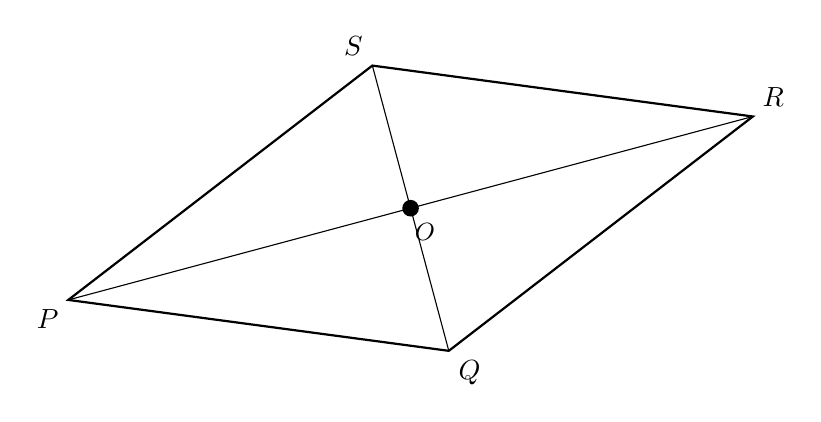
\begin{tikzpicture}[scale=1.5]
    % Define the center point O
    \coordinate (O) at (0,0);

    % Define vertices based on diagonal lengths (PR = 24, QS = 10)
    % We scale them down (e.g., divided by 4) for drawing purposes
    % Diagonal PR (horizontal-ish): 24 / 4 = 6 units total (3 units from center)
    % Diagonal QS (vertical-ish): 10 / 4 = 2.5 units total (1.25 units from center)
    % A small rotation is added to match the visual orientation in the image
    \begin{scope}[rotate=15]
        \coordinate (P) at (-3, 0);
        \coordinate (R) at (3, 0);
        \coordinate (S) at (0, 1.25);
        \coordinate (Q) at (0, -1.25);
    \end{scope}

    % Draw the rhombus sides
    \draw[thick] (P) -- (Q) -- (R) -- (S) -- cycle;

    % Draw the diagonals crossing at O
    \draw (P) -- (R);
    \draw (Q) -- (S);

    % Labels for vertices
    \node[below left] at (P) {$P$};
    \node[below right] at (Q) {$Q$};
    \node[above right] at (R) {$R$};
    \node[above left] at (S) {$S$};
    
    % Label for intersection O
    \node[below right=2pt and -2pt of O, font=\small] {$O$};

    % Small dot at the intersection
    \fill (O) circle (2pt);
\end{tikzpicture}